\section{Abstractions for NDA}
\label{sec:abstractions}

\begin{quote}
{\em Synthesis implies a bridge between two layers of abstraction} -- A. Sangiovanni-Vincentelli~\cite{alberto}
\vspace{-2mm}
\end{quote}

\begin{figure}[t]
\centerline{
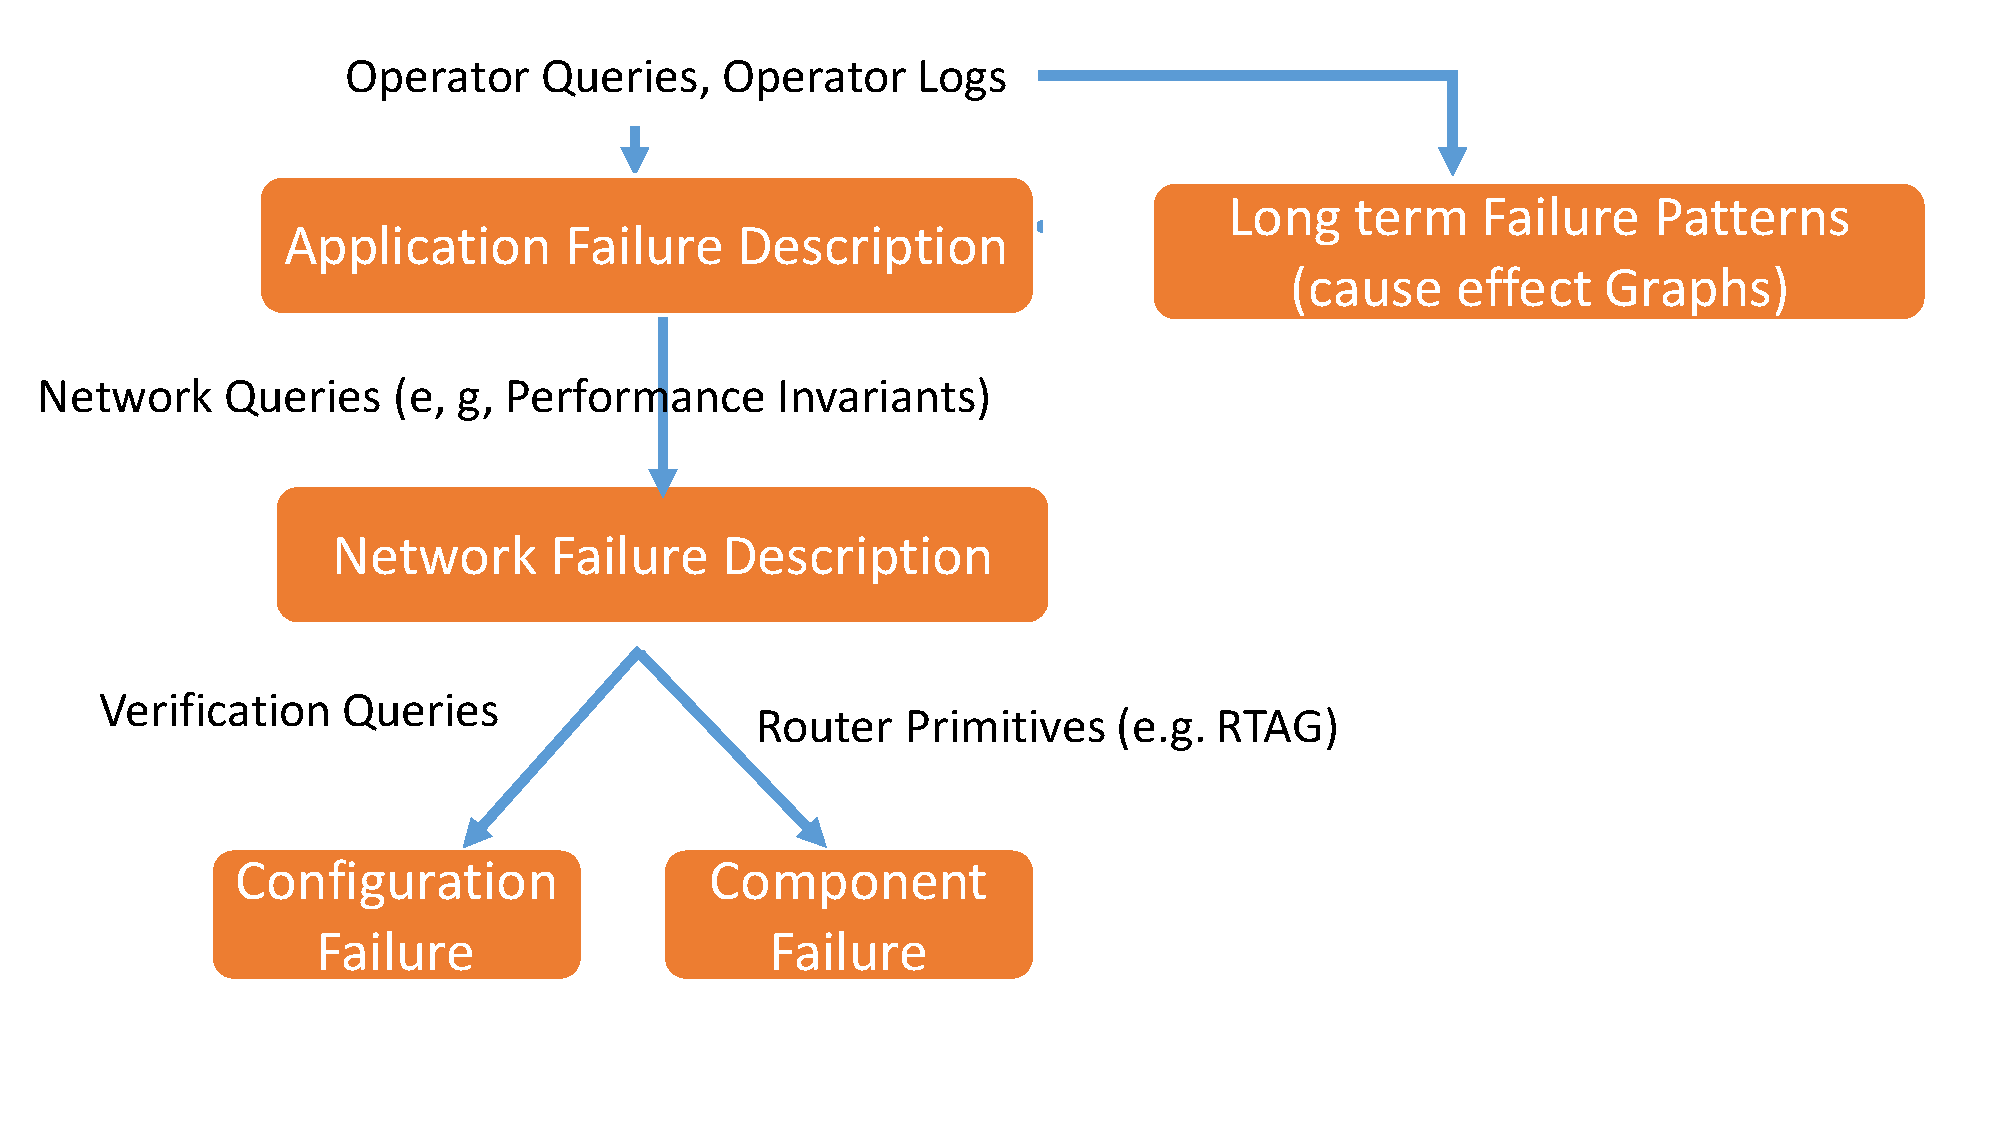
\epsfig{file=NDA-abstractions-new.pdf, height=4in}
}
\caption{\label{fig:abstractions} The layers of abstraction in NDA.}
\vspace{-5mm}
\end{figure}

Abstractions were key to the success of EDA~\cite{malik}. By steadily
raising the level of abstraction for designers, EDA allowed complex
chip designs to be developed using high-level behavioral models that
are mapped to blocks, to logic gates, and finally to lists of
wires. Although early efforts in EDA focused on bottom-up
verification, later innovation allowed synthesis between abstraction
levels.

\paragraph*{Abstractions for NDA}
%
Our proposal seeks to develop an analogous but preliminary set of \emph{interconnected} abstractions for NDA in the specific thrusts of synthesis and debugging. Networks already have
abstractions for packet delivery (TCP and IP~\cite{kurose}) and for
packet forwarding (SDN-inspired flow
rules~\cite{Ethane,4DControlPlane,shenker-abstractions}) but do not have interconnected abstractions for
designing and configuring the network, and for debugging at a systems level.

The two abstraction levels for synthesis are fairly straightforward: topology and configuration. 
The first level abstraction is a {\em network topology}.  In our vision, each
abstraction layer corresponds to a tool.  For example, we envision a topology tool wherein an architect specifies traffic growth forecasts, resiliency requirements and components like routers and links, and the tool produces the physical network.  Many cloud providers including Google~\cite{condor} and Microsoft already have such tools but these are proprietary and would not apply to a rural network like MoTech.  

Imagine an open source tool that can design a physical network whether
for a rural network that uses VoIP (1000 users in 12 villages, using wireless links and FPGA based routers) or a larger data center network for Google (10, 000 users for Google Applications using high end Cisco routers) or a CDN. The Condor system at
Google~\cite{condor} recently proposed a delarative Topology
Description Language (TDL) to specify abstract topology connectivity
and uses a constraint solver to generate topologies but it only automates
some limited aspects of topology design.

The next layer of abstraction is a description of the configuration at each router in the topology as specified
by a Configuration Description Language (CDL).  There are candidates for such a CDL already such as 
Open Config~\cite{openconfig}, Yang~\cite{yang}, and the intermediate representation in the open-source Batfish~\cite{batfish} tool that PI Millstein has worked on.  Imagine an open source scripting tool that 
can convert higher level policy intent by an operator to a CDL down and then map them to vendor specific
configurations such as Cisco or Juniper. Taken together, topology and configuration synthesis comprise our
first thrust. Note that while synthesis maps fronm policy to configuration, we will also deepen work in verification tasks that map from configuration to policy for existing networks.

Next, note that when an architect (statically) synthesizes a network, the performance envelope of the 
network is known (modulo a set of common failures) but there are always properties that cannot be verified during synthesis  (especially unexpected events and failures beyond the expected failures the synthesis
consider). Thus one needs systems level debugging and instrumentation in the network and a set of
interconnected abstractions that ties these levels of debugging together, which is our second thrust.

For systems level debugging, we have identified an initial set of layers of
a network that will frame our proposed debugging research
(Figure~\ref{fig:abstractions}): {\em application failure description}, {\em network failure description}, ,  
{\em configuration failure description}, and {\em component failure description}.  The idea is to map 
from the highest layer (application failures) to lower level culprits (configurations, components) by a set
of interconnected tools.

First, note that higher level operator concerns and problems are often expressed in operator logs.  While
we will also design a language to express operator concerns (e.g., SLA violations), we feel it is also
important to map from operator logs to application problems ( using Natural Language Processing.
Next, we need connecting the abstract, high-level application failure language to the
low-level, structured query languages that express network failures (e.g., Marple~\cite{marple} or 
our proposal for  performance invariants).  Finally, we isolate the issue when possible to 
either a configuration failure (that can be detected by configuration verification tools (e.g., Minesweeper\cite{minesweeper} or enhacements we describe later) or router primitives (e.g., packet mirroring as in
Everflow or RTAG as we describe later).

 On a longer time scale, the
network architect needs to extract, from logs of network faults
captured (often annotated by a network operator), a higher-level
{\em failure model}, which can be used to target efforts to improve
reliability. We lump all these concerns into the bottommost level


Section~\ref{sec:approaches} describes our proposed work to map between abstraction levels
in detail and sets it in the context of related work.

% In the following paragraphs, we discuss our
% research in synthesis and verification, achieved through pairwise
% inter-disciplinary collaborations.


Notice that our tools work on designing specialized networks within a single
Autonomous Systems or AS where the architect and operator can control the 
entire network.  Examples include rural networks, data center networks ad 
enterprise networks. Of course, individual networks are interconnected to form the Internet .  We do not focus on such Network Design Automation ``in the large''
because we feel that is precisely the specialized context (rural networks, 
data center networks) that can allow novel language based synthesis and
verification tools to work.

\paragraph*{Our Approach:} While there exist point solutions at some of
these layers for certain tasks, these abstractions are neither {\em
  complete} or {\em interconnected}. We will produce a complete and
interconnected set of abstractions from topology down to schedules.
Interconnecting abstractions allows us to build
an end-to-end system for rural networks, as we propose
in our evaluation.



 
